%%% There's not a lot of extra documentation in this file, other than
%%% the text itself.  On the other hand, you may be looking for
%%% a few examples of how to insert figures, so go ahead and peruse.

\chapter{Working with Graphics}

In this chapter, we'll be dealing with the inclusion and placement of
figures and other graphics in your thesis.  Usually a figure will be a
graphic of some type (e.g., a photograph, line drawing, chart) that
resides in a separate file external to your document.  You will need
to decide on a format for these figures.  If you are generating your
own graphics using other programs, you may have the option to choose
the output format.  Otherwise, you may need to use other software to
convert the graphic into a compatible format for inclusion in your
\LaTeX{} document.

\section{Raster and Vector Graphics}
Graphics for print media are generally in one of two classes: raster
images or vector drawings.  A \acro{JPEG} photograph is an example of
a raster format, where a matrix of pixels has a defined value.  Raster
images may be scaled up or down in size, but within limits. Scale such
an image too large and it will become ``pixelated'' or blocky.
Reduce the image too much, and finer details will be blurred or lost.
If you use raster images in your thesis, they should be generated with
a sufficiently high resolution that scaling artifacts will be
minimized.  For print media, a resolution of 300 to 600\,dpi (dots per
inch) might be typical.  For viewing on screen, a minimum resolution
of 100\,dpi may be adequate.  \acro{PNG}, \acro{JPEG} and \acro{GIF}
images are common examples of a raster type.  PhotoShop, The Gimp, and
other paint-type or photo-manipulation programs typically generate
raster images.  Scanning documents or other graphics will also
generate a raster image of some kind, usually in one of \acro{JPEG},
\acro{TIFF}, or \acro{PDF} formats.

In contrast, vector images will scale better.  Vector images are
usually line-drawings, text, and many kinds of graphs.  Vector images
can be scaled better because the pixel values are not defined until
after the scaling occurs, so the image can be rendered at the full
resolution of the output device, whether it be for print or screen.
Also, vector images are often encoded in a much smaller space than a
comparably-sized raster image.  Adobe Illustrator, CorelDRAW,
Inkscape, and Flash are examples of programs that generate vector
images.  \acro{WMF} and \acro{SVG} are also common vector formats,
though these may not be included in your documents directly.

In generating figures, if you have a choice, choose a vector format,
since it will provide the best scaling flexibility.  However, if you
must include a photograph or scanned document of some type, then be
sure that the raster image has a sufficiently high resolution for the
intended publishing medium.

\section{The \pkg{graphicx} Package}
The \LaTeX{} package \pkg{graphicx} allows you to insert external
PostScript or other files into your document.  There are other
figure-inclusion packages that you can use, but \pkg{graphicx} is
probably the most common for the task.

This main document file has a \verb|\usepackage[dvips]{graphicx}| line
in order to include figures.  The option \lit{dvips} indicates that
the \pkg{graphicx} package should employ the PostScript driver for the
program \lit{dvips} (which converts \LaTeX's standard \acro{DVI}
output into PostScript).  Using this driver, all your external figures
will need to be in Encapsulated PostScript (\acro{EPS}) form.  Other formats
will need to be first converted to PostScript.  (Both PostScript and
\acro{PDF} formats may contain either raster or vector images, or even
both at once.)

An alternative driver to \lit{dvips} is the option \lit{pdftex}, which
will require all your figures to be in \acro{PDF}, \acro{JPEG}, or
\acro{PNG} format.  This will be the preferred driver if you intend to
use \lit{pdflatex} to generate your document in \acro{PDF} form
directly, rather than going through an intermediate PostScript form
first.  All the figures in this document (found in the \lit{figures}
directory) are available in both \acro{EPS} and \acro{PDF} formats, so
you may use either driver.  In fact, there's some fancy code in the
\lit{thesis.tex} file that chooses the right driver depending on whether
you're running \lit{pdflatex} or \lit{latex} to process this document.

\section{PostScript and Encapsulated PostScript}
PostScript is a programming language for putting marks on a page.  As
such, PostScript files can usually be edited using plain text editors,
should that ever be necessary.  A file containing Encapsulated
PostScript conforms to additional standards, allowing the graphic to
be manipulated or included in other PostScript programs more readily.
Encapsulated PostScript is the preferred format for use with \LaTeX.

As far as \LaTeX{} is concerned, the most important feature of an
Encapsulated PostScript file is the \lit{\%\%BoundingBox}, which is
defined as the smallest rectangle that completely encloses the figure.
Two sets of $x$- and $y$-coordinates describe the bounding box; the
first $(x,y)$ pair gives the lower left-hand coordinates of box
relative to the bottom left-hand corner of the page, and the second
pair of coordinates identify the upper right-hand corner of the
bounding box.  You normally don't have to worry about this information
at all, but if a PostScript figure does not contain
\lit{\%\%BoundingBox} information, or if the \lit{\%\%BoundingBox} is
incorrect, the \pkg{graphicx} package allows you to specify the
bounding box coordinates yourself when you insert the figure into your
document.

Depending on your distribution of \LaTeX, you may have a program
already installed which converts \acro{EPS} files to \acro{PDF}.
One of the simplest converters is the program \lit{epstopdf}, which
can be executed as follows:
\begin{verbatim}
epstopdf myfig.eps
\end{verbatim}
A Windows version of this program might pop up a user interface for
fine-tuning the figure conversion, while the Unix/Linux version of the
program will simply do the conversion, creating \lit{myfig.pdf}
without any intervention required.

\section{Inserting Figures}
The basic mechanics of including a PostScript graphic (\lit{dvips}
driver) or \acro{PDF} graphic (\lit{pdftex} driver) are relatively
simple:
\begin{verbatim}
\includegraphics{figurefile}
\end{verbatim}
This command will insert the graphic contained in the file
\lit{figurefile} at that particular location in the text.  The file
name may have optional extensions, depending on the driver.  For
example, the \lit{dvips} driver will recognize the \lit{.ps} or
\lit{.eps} file extensions, while the \lit{pdftex} driver will
recognize extensions \lit{.pdf} and \lit{.jpg}.  \LaTeX{} will leave
space for the graphic according to the bounding box information that
the file contains.

For inclusion in your thesis or dissertation, a graphic will normally
be labeled and given a caption.  To do this, you will wrap the
\verb|\includegraphics| command in a \lit{figure} environment.
Figures will usually ``float'' from the location where they were
defined.  By default, \LaTeX{} will try to place figures at the bottom
of the current page (if there's sufficient room), then at the top of
the next available page.  Failing that, \LaTeX{} will place figures
onto their own page.  The \verb|\caption| command will number the
figure automatically.  If you need to refer to the figure in your
text, include a \verb|\label| command following the \verb|\caption|,
and then use the \verb|\ref| and \verb|\pageref| commands to
retrieve the figure number and figure's page number, as required.

As a complete example, refer to Figure~\ref{ex-complete}.  I used the
following commands to include the figure graphic:
\begin{verbatim}
\begin{figure}
\begin{center}

\includegraphics{figures/fleur}
\end{center}
\caption{This is a simple figure, but a complete example.}
\label{ex-complete}
\end{figure}
\end{verbatim}
In this case, the graphic file is located in the folder \lit{figures},
and the complete file name is either \lit{fleur.eps} or
\lit{fleur.pdf}. If I'm using the \lit{dvips} driver, the \lit{.eps}
extension is added automatically; likewise, the \lit{.pdf} extension
would be added if I am using the \lit{pdftex} driver.  In order to
center the graphic horizontally, I enclosed the
\verb|\includegraphics| command in a \lit{center} environment. The
\verb|\caption| command will handle its text in its own way: a short
caption will be horizontally-centered, and a longer caption will be
broken into multiple lines as required.  At the beginning of the
paragraph, I typed \verb|Figure~\ref{ex-complete}| to refer to the
figure number.  Using this mechanism, I never have to worry about
renumbering my figures if I choose to move text or figures around.  I
can also tell you that Figure~\ref{ex-complete} will be found on
page~\pageref{ex-complete} by typing
\begin{verbatim}
Figure~\ref{ex-complete} will be found on page~\pageref{ex-complete}
\end{verbatim}

\begin{figure}
\begin{center}

\includegraphics[scale=0.75]{figures/fleur}
\end{center}
\caption{This is a simple figure, but a complete example.}
\label{ex-complete}
\end{figure}

The \verb|\includegraphics| command has several optional arguments
which will allow you to adjust figure position, bounding box,
rotation, scaling, and other elements, without having to edit the
figure itself.  Figure~\ref{franklin} displays an image in its raw
state, and then a close-up, rotated image of a segment of the same
PostScript graphic.  A complete description of the all the options
available is best left for the \pkg{graphicx} package manual page, but
the transformed image was accomplished with the following
\verb|\includegraphics| line:
\begin{verbatim}
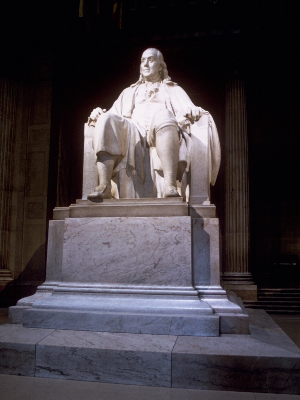
\includegraphics[viewport=.9in 2.1in 1.15in 2.35in,clip,
    scale=10.67,angle=90]{figures/ben}
\end{verbatim}

\begin{figure}
\begin{center}
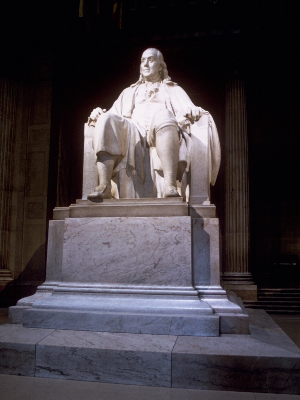
\includegraphics{figures/ben}
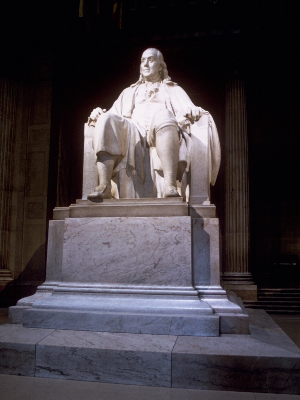
\includegraphics[viewport=.9in 2.1in 1.15in 2.35in,clip,
    scale=10.67,angle=90]{figures/ben}
\end{center}
\caption{Benjamin Franklin, in raw form (left), and close-up and
  rotated (right).  (Notice that the close-up figure displays
  ``pixelation'' effects of a raster image scaled too large.)}
\label{franklin}
\end{figure}

\section{Musical Examples}
If your thesis or dissertation requires you to include musical
examples, the \pkg{fsuthesis} class has an environment already set up
for you.  Each musical example should be in its own PostScript
\acro{EPS} file or \acro{PDF} file (depending on the \pkg{graphicx}
driver you are using).  Then, rather than using the \lit{figure}
environment, you would use the \lit{musex} environment as demonstrated
here to create Example~\ref{mus:bass-ode}:
\begin{verbatim}
\begin{musex}
\begin{center}
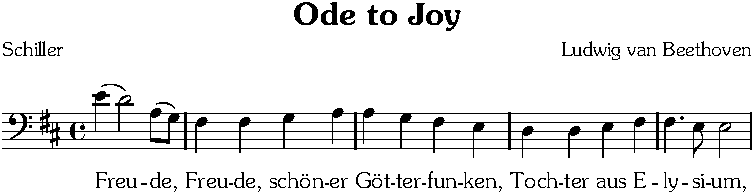
\includegraphics{figures/freude}
\end{center}
\caption{The bass soloist's opening statement in the 9th Symphony.
  \label{mus:bass-ode}}
\end{musex}
\end{verbatim}

As with figures, the caption follows the graphic.  However, the
caption will be automatically titled with ``Example'' rather than
``Figure''.  If your document contains more than one musical example,
they can be listed in their own table by using the command
\verb|\listofmusex| in the front matter section of your document.

\begin{musex}
\begin{center}
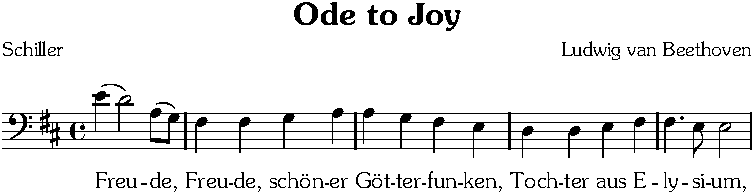
\includegraphics{figures/freude}
\end{center}
\caption{The bass soloist's opening statement in the 9th Symphony.
\label{mus:bass-ode}}
\end{musex}

\section{Further Information}
This chapter intended to provide a brief overview of figure inclusion,
along with a few simple examples.  If your figure-insertion needs have
not yet been addressed, you should look up the document \textit{Using
  Imported Graphics in \LaTeX{} and pdf\LaTeX} by Keith Reckdahl,
which is part of the Comprehensive \TeX{} Archive Network (CTAN).
This document provides a wealth of detail about figure manipulation,
insertion, and placement.

In addition to the inclusion of external figures, \LaTeX{} provides
several environments and packages for creating figures mathematically
within a \LaTeX{} document itself, usually technical line-drawings.
Investigate the \pkg{picture} package and its extensions \pkg{epic}
and \pkg{eepic}.  Other figures and text manipulations can be carried
out with the \pkg{pstricks} package.  The program \MP{} can generate
precise renderings of mathematical objects and diagrams.  And there
are many more utilities and packages to assist you.

